%
% File acl2017.tex
%
%% Based on the style files for ACL-2015, with some improvements
%%  taken from the NAACL-2016 style
%% Based on the style files for ACL-2014, which were, in turn,
%% based on ACL-2013, ACL-2012, ACL-2011, ACL-2010, ACL-IJCNLP-2009,
%% EACL-2009, IJCNLP-2008...
%% Based on the style files for EACL 2006 by 
%%e.agirre@ehu.es or Sergi.Balari@uab.es
%% and that of ACL 08 by Joakim Nivre and Noah Smith

\documentclass[11pt,a4paper]{article}
\usepackage[hyperref]{acl2017}
\usepackage{times}
\usepackage{latexsym}
\usepackage{graphicx}
\usepackage{booktabs}
\usepackage{amsmath}
\usepackage{todonotes}
\usepackage{multirow}
\usepackage{enumitem}
\usepackage{amsfonts}
\usepackage{url}

\aclfinalcopy % Uncomment this line for the final submission

\makeatletter
\newcommand{\@emptybiblabel}[1]{}
\makeatother
\DeclareMathOperator*{\argmax}{arg\,max}
%\setlength\titlebox{3.5cm}    % Expanding the titlebox

\newcommand*{\checktikz}[1][]{\tikz[x=1em, y=1em]\fill[#1] (0,.35) -- (.25,0) -- (1,.7) -- (.25,.15) -- cycle;}
\newcommand*{\crosstikz}[1][]{\tikz[x=1em, y=1em]\fill[#1] (0,0) -- (1,1) -- (0.5,0.5) -- (0.1,0.1) -- cycle;}

\newcommand\BibTeX{B{\sc ib}\TeX}
\newcommand{\Correct}{\checktikz[draw=black]}
\newcommand{\ValidMiss}{\checktikz[draw=gray,fill=white]}
\newcommand{\Valid}{\checktikz[draw=gray,fill=white]}
\newcommand{\Missed}{\checktikz[draw=black]} %\textsf{X}~}
\newcommand{\Wrong}{} %\textsf{X}~}

\newcommand{\U}{\mathbb{U}}

\author{Sudha Rao, Hal Daum\'e III \\
  Department of Computer Science \\
  University Of Maryland, College Park \\
  {\tt raosudha@cs.umd.edu, hal@cs.umd.edu}}

\title{Are you asking the right questions? \\ Teaching Machines to Ask Clarification Questions}

\date{}

\begin{document}
\maketitle
\begin{abstract}
Inquiry is fundamental to communication, and machines cannot effectively collaborate with humans unless they can ask questions. 
%We explore how can a machine automatically generate clarification questions when faced with uncertainty, a task of increasing importance in today's automated society. 
We study the problem of question generation using data from StackExchange, a plentiful online resource in which people routinely ask clarifying questions to posts so that they can better offer assistance to the original poster. We build neural network models inspired by the idea of the expected value of perfect information: a good question is one whose expected answer is going to be most useful. Our results demonstrate significant improvements by modeling the value of information.
\end{abstract}

\section{Introduction}\label{introduction}

A main goal of asking questions is to fill information gaps, typically through clarification questions, which naturally occur in conversations. 
A good question is one whose \emph{likely answer} is going to be most useful.
Consider the exchange in Figure~\ref{askubuntu_post}, in which an initial poster (who we'll call ``Terry'') asks for help configuring environment variables.
This question is underspecified and a responder (``Parker'') asks a clarifying question ``\textsf{\small (a) What version of Ubuntu do you have?}''
Parker could alternatively have asked one of:

\textsf{\small(b) Is the moon waxing or waning?}

\textsf{\small(c) Are you running Ubuntu 14.10 kernel 4.4.0-59-generic on an x86\_64 architecture?}

\noindent
Parker should not ask (b) because it's not useful; they should not ask (c) because it's too specific and an answer of ``No'' gives little help.
Parker's question (a) is optimal: it is both likely to be useful, and is plausibly answerable by Terry.
Our goal in this work is to automate Parker.
Specifically, after Terry writes their initial post, we aim to generate a clarification question so that Terry can immediately amend their post in hopes of getting faster and better replies.
\begin{figure}[!t]
	\centering
	\setlength\fboxsep{1pt}
	\setlength\fboxrule{0.5pt}
	\fbox{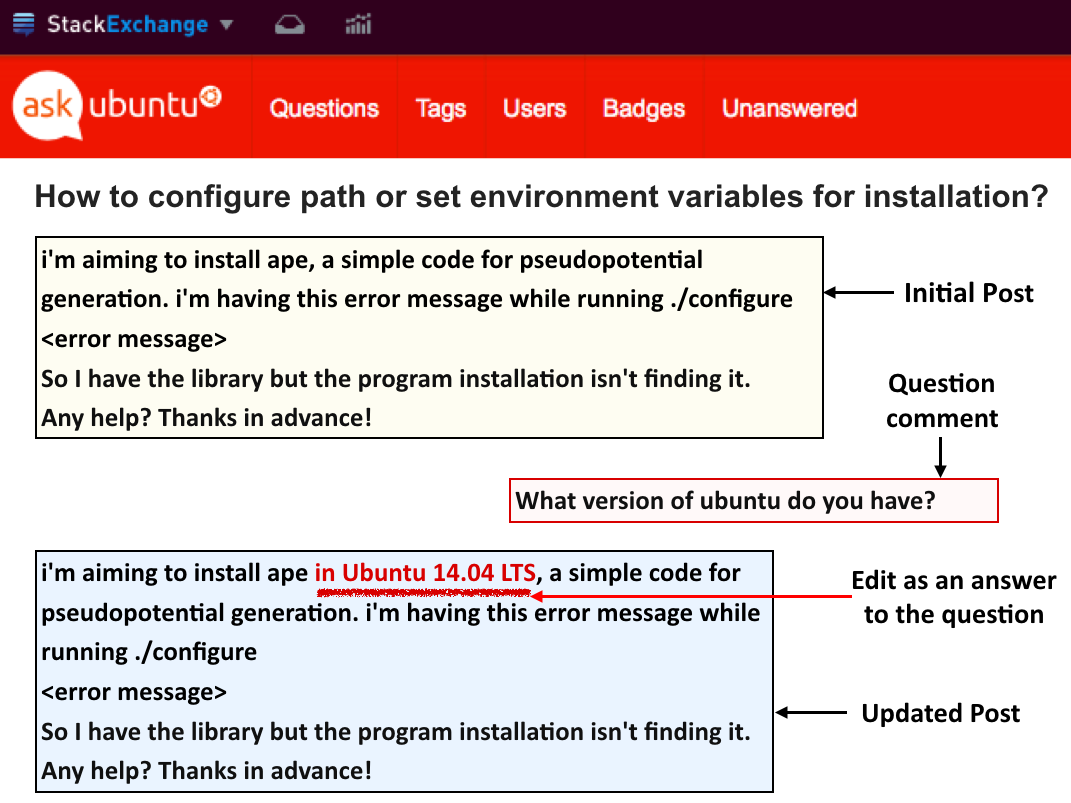
\includegraphics[width=0.47\textwidth]{askubuntu_post}}
	\caption{A post on an online Q \& A forum ``askubuntu.com'' is updated to fill the missing information pointed out by the question comment}
	\label{askubuntu_post}
\end{figure}
%
Our work has two main contributions: 
\begin{enumerate}[noitemsep,nolistsep]
	%\item Identifying the problem of generating clarification questions as a problem worth of study, both in its own right and as part of the larger problem of building naturalistic conversational systems. 
	\item A novel neural-network model for addressing this task that integrates the notion of expected value of perfect information (\S\ref{model_description}). % , a classic formalization from AI
	\item A novel dataset, derived from StackExchange, that enables us to learn a model to ask clarifying questions by looking at the types of questions people ask (\S\ref{dataset_creation}). %\footnote{We use data from StackExchange; per license cc-by-sa 3.0, the data is ``intended to be shared and remixed'' (with attribution). We will release all of the data we extract.}
\end{enumerate}

\begin{figure*}[t]
	\centering
	\includegraphics[width=0.85\textwidth]{model_description}
	\caption{\small The behavior of our model during test time. Given a post $p$, we use Lucene to retrieve 9 posts similar to post $p$ and consider the questions asked to those 9 posts, plus the original, as question candidates $Q$ and the edits made to the posts in response to the questions as our answer candidates $A$. For each question candidate $q_i$, we generate an answer representation $F(p,q_j)$ and model the answer probability $\mathbb{P}[a | p,q]$ as the closeness of the answer candidate $a_k$ to the answer representation $F(p,q_j)$. The utility function $U$ calculates the utility of the post if it were updated with the answer $a_k$. Finally we return the question $q$ that maximizes the expected utility of the post $p$ (Equation~\ref{evpi_equation}).}
	\label{model}
\end{figure*}

\section{Related Work}
The problem of question generation has received sparse attention from the natural language processing community. Most prior work focuses on generating reading comprehension questions \cite{vanderwende2008importance,penas2010filling,heilman2011automatic}: given text, write questions that one might find on a standardized test. Comprehension questions, by definition, are answerable from the provided text. Clarification questions are not. Outside reading comprehension questions, \newcite{labutov2015deep} studied the problem of generating question templates via crowdsourcing, \newcite{liu2010automatic} use template question generation to help authors write better related work sections, \newcite{mostafazadeh2016generating} consider question generation from images, and  \newcite{artzi2011bootstrapping} use human-generated clarification questions to drive a semantic parser.

\section{Model Description}\label{model_description}

In order to choose what question to ask, we build a neural network model inspired by the theory of expected value of perfect information (EVPI). EVPI is a measurement of: if I were to acquire information X, how useful would that be to me? However, because we haven't acquired X yet, we have to take this quantity in expectation over all possible X, weighted by each X's likelihood. In the question generation setting, for any given question $q$ that we can ask, there is set $A$ of possible answers that could be given. For each possible answer $a \in A$, there is some probability of getting that answer, and some utility if that were the answer we got. The value of this question $q$ is the expected utility, over all possible answers. The theory of EVPI then states that we want to choose the question $q$ that maximizes:
\begin{equation}\label{evpi_equation}
\argmax_{q \in Q} \sum_{a \in A} \mathbb{P}[a | p,q] \U(p+a)
\end{equation} 

In Eq~\ref{evpi_equation}, $p$ is the post, $q$ is a potential question from a set of candidate questions $Q$ (\S\ref{question_candidate_generator}) and $a$ is a potential answer from a set of candidate answers $A$ (\S\ref{question_candidate_generator}). $\mathbb{P}[a | p,q]$ (\S\ref{answer_modeling}) measures the probability of getting an answer $a$ given an initial post $p$ and a clarifying question $q$. $\U(p+a)$ (\S\ref{utility_calculator}) measures how useful it would be if $p$ were augmented with answer $a$. Finally, using these pieces, we build a joint neural network that we can optimize end-to-end over our data (\S\ref{neural_network}). Figure~\ref{model} describes the behavior of our model during test time. 

\subsection{Question \& Answer Candidate Generator}\label{question_candidate_generator}

Given a post, we first identify 10 posts similar to the given post in our dataset using Lucene\footnote{\url{https://lucene.apache.org/}} and consider the questions asked to these posts as our set of question candidates and the edits made to the posts in response to the questions as our set of answer candidates.

\subsection{Answer Modeling}\label{answer_modeling}

Given a post $p$ and a question candidate $q_i$, we calculate the probability of this question being answered using one of our answer candidates $a_k$ by measuring how close is the answer candidate $a_k$ to our answer representation $ F_{ans}(p,q_i)$ :
\begin{align}
\mathbb{P}[a_k |p,q_i]  
&= \frac 1 Z \exp\left[- \lambda || a_k  -  F_{ans}(p,q_i) ||^2\right]
\end{align}
where $\lambda$ is a tunable parameter that controls the variance of the distribution. We train our answer representation $ F_{ans}(p,q_i)$ to be close to the true answer $a_i$ paired with question $q_i$ and close to the answer $a_j$ corresponding to a question $q_j$ very similar to $q_i$ using the loss function below:
\begin{align}\label{eq_answer_generator}
\textrm{loss}_{\textrm{ans}}(\bar p, \bar q, \bar a, Q) 
&=  {|| F_{ans}(\bar p, \bar q) - \bar a||}^2 & \\
&\hspace{-28mm} +  \sum_{j \in Q} \Big ( {|| F_{ans}(\bar p, \bar q) - \bar{a_j} ||}^2  (1 - \tanh{(|| \bar q - \bar{q_j} ||^2)}) \Big ) &\nonumber
\end{align}

\begin{table}[t]
	\small
	\centering
	\begin{tabular}{l|cccc|}
		\toprule
		\textbf{Models} & Acc & MRR & R@3 & R@5\\
		\midrule
		Random  & 10.0 & 29.3 & 30.0 & 50.0  \\
		Bag-of-ngrams & 11.6 & 31.3 & 32.5 & 54.6  \\
		Feed-forward & 17.4 & 37.8 & 43.2 & 63.9  \\
		EVPI & \bf 23.3 & \bf 43.4 & \bf 51.0 & \bf 70.3 \\
		\bottomrule
	\end{tabular}
	\caption{\small Results on askubuntu test set when trained on a combination of three domains: askubuntu, unix and superuser.  We report four metrics: accuracy (percent of time the top ranked question was correct),
		mean reciprocal rank (the reciprocal of the ranked position of the correct question in the top 10 list), recall at 3 (percent of time the correct answer is in the top three) and
		recall at 5.}
	\label{tab:results_topN}
	\vspace{-1.0em}
\end{table}

\subsection{Utility Calculator}\label{utility_calculator}
We calculate the utility of the updated post $\U(p + a_k)$ using the intuition that a post $p_i$, when updated with the answer $a_i$ that it is paired with in our dataset, would be more complete than if it is updated with some other answer $a_j$. Therefore we label all the $(p_i, a_i)$ pairs from our dataset as positive ($y=1$) and label $p_i$ paired with other nine answer candidates generated using Lucene (\S\ref{question_candidate_generator}) as negative ($y=0$). The utility of the updated post is defined using a feedforward neural network $F_{utility}$ which is trained to be close to one for all the positively labelled $(p,a)$ pairs and close to zero for all the negatively labelled $(p, a)$ pairs using the loss function below:
\begin{align}\label{eq_utility_calculator}
\textrm{loss}_{\textrm{util}}(y, \bar p, \bar a) &= y \log(\sigma (F_{utility}(\bar{p}, \bar{a})))
\end{align}

\subsection{Our joint neural network model}\label{neural_network}
Our fundamental representation is based on long short-term memory architecture (LSTM) \cite{hochreiter1997long} over word embeddings obtained using a GloVe \cite{pennington2014glove}. We define three LSTMs corresponding to $p$, $q$ and $a$ and two feedforward neural networks corresponding to our answer model $F_{ans}(\bar{p},\bar{q})$ and our utility calculator $F_{utility}(\bar{p}, \bar{a})$. We jointly train the parameters of all our neural network models to minimize the sum of the loss of our answer model (Eq~\ref{eq_answer_generator}) and our utility calculator (Eq~\ref{eq_utility_calculator}):
%
\begin{align}
\sum_i \textrm{loss}_{\textrm{ans}}(\bar p_i, \bar q_i, \bar a_i, Q_i)  
+  \textrm{loss}_{\textrm{util}}(y_i, \bar p_i, \bar a_i)
\end{align}
%
Given such an estimate $\mathbb{P}[a|p,q]$ of an answer and a utility $\U(p+a)$ of the updated post, we do predictions by choosing that ``$q$'' that maximizes Eq~\ref{evpi_equation}. 

\section{Dataset creation}\label{dataset_creation}

 We train our models using $(p,q,a)$ triples that we extract automatically from StackExchange.
Figure~\ref{askubuntu_post} depicts how we do this using StackExchange's edit history.  In the figure, the initial post fails to state what version of Ubuntu is being run. In response to the clarification question in the comments section, the author of the post edits the post. We extract the initial post as $p$, question posted in the comments section as $q$, and edit to the original post as answer $a$ to form our $(p,q,a)$ triples. We extract a total of 37K triples from the following three domains of StackExchange: askubuntu, unix and superuser.

\section{Experiments and Results}

\subsection{Experimental Setups}\label{task_setup}
We define our task as given a post and 10 question candidates, select the correct question candidate. For every post $p$ in our dataset of $(p, q, a)$ triples, the question $q$ paired with $p$ is our positive question candidate the nine question candidates retrieved using Lucene  (\S\ref{question_candidate_generator}) are our negative candidates.

\subsection{Baseline Methods}\label{baselines}

\textbf{Random}: Randomly permute the set of 10 candidate questions uniformly.\\
\textbf{Bag-of-ngrams}: Construct a bag-of-ngrams representation for the post, the question and the answer and train a classifier to minimize hinge loss on misclassification loss. \\
\textbf{Feed-forward neural}: Concatenate the post LSTM representation, the question LSTM representation and the answer LSTM representation and feed it through a feed forward neural network of two fully-connected hidden layers.

\subsection{Results}

We describe results on a test split of askubuntu when our models are trained on the union of all data, summarized in Table~\ref{tab:results_topN}. Here, we see that for all the evaluation metrics, EVPI outperforms all the baselines by at least a few percentage points. A final performance of 51\% recall at 3 in the ``hard'' setting is encouraging, though clearly there is a long way to go for a perfect system. 

%We additionally compare the performance of our model with that of non-expert humans and find that human performances, although much better than our model, is still far from perfect suggesting the high level of difficulty of this task. 
%There are three main avenues for improvement of this work. 
%The first is in evaluation: given that this task is so difficult for humans, but also given that there is no single right question to ask, how can we better measure performance at this task?
%Second, to make question generation more general, systems need to be able to generalize, for instance by constructing templates of the from ``What version of \_\_\_ are you running?'' into which the system would need to fill a variable. 
%Finally, asking question is a natural component of dialog, and building a collaborative dialog system that can naturally converse with a user is a broad long term goal.

\bibliography{acl_winlp}
\bibliographystyle{acl_natbib}

\end{document}
